Section \ref{sec:traditional-distributed-computing} described the traditional
distributed computing model, where the service provider is trusted by the data
owner, and defined a generalized layered model. This chapter will define a
threat model, identify threats and issues of the Infrastructure and Platform
layers when the service provider becomes untrusted. Subsequently, the new
trusted distributed computing model will be defined, by integrating TEE
technology (see Section \ref{sec:confidential-computing}) and the RATS framework
(see Section \ref{sec:remote-attestation}) into the traditional distributed
computing model. Finally, this chapter demonstrates this new model by looking at
two case studies and evaluates the new model based on the threat model.

\section{Threat Model}
\label{sec:untrusted-threat-model}

\subsection{Infrastructure Layer}

\begin{description}
  \item[Threats from storage resources]
    Storage resources of the Infrastructure layer are typically protected by
    physically securing the location of the hardware and application transparent
    encryption. However, in the trusted distributed computing model the
    service provider is untrusted, and the application owner has to implement
    application level encryption, preventing the service provider gaining plain
    text access to confidential data.

  \item[Threats from networking resources]
    Networking resources offer means of communication. However, in a distributed
    computing environment, these communication channels are often untrusted as
    these resources are shared between multiple tenants. An attacker might gain
    unauthorized access to confidential data shared by an application by
    capturing data from the shared network resources. Applications sharing
    confidential data using untrusted communication channels need to implement
    authentication \cite{lampson1992authentication}, authorization
    \cite{woo1992authorization}, and encryption in order to securely use these
    untrusted communication channels and not leak confidential data to a
    malicious attacker that has access to network resources. Authentication and
    encryption is usually implemented using the Transport Level Security (TLS)
    protocol \cite{rfc5246}, which utilizes a trusted third party (the
    certificate authority) for authentication and the Diffie-Hellman key
    exchange protocol in order to establish a shared secret for encryption.

    Typically, these implementations do not rely on services provided by the
    service provider and as such pose no issues for moving to an untrusted
    distributed computing model.

  \item[Threats from compute resources]
    Techniques for protecting data resting in storage and traversing networking
    resources largely are based on cryptographic primitives, such as encryption,
    one-way hash functions, and digital signatures. All of these primitives
    require some kind of cryptographic key (e.g. secret key for symmetrical
    encryption, private keys for asymmetrical encryption and singing) that need
    to be kept secret. Typically, these keys and the decrypted data are stored
    unprotected in the memory of the machines while in use and is therefore a
    prime target for attacks.

    There are two types of physical attacks, related to the memory of a system,
    summarized by \citeauthor{weis2014protecting} \cite{weis2014protecting}:
    \textsb{Direct Memory Access (DMA) Attacks} exploit the design of the x86
    instruction set architecture that allow hardware subsystems to bypass the
    CPU and directly access the memory of the machine. Like the name implies,
    \textsb{Physical Memory Extraction (PME) Attacks} directly extract data from
    the physical system memory of a machine. Example for this type of attack are
    monitoring the memory bus of a machine, cold boot attacks, and exploiting
    special persistent, nonvolatile memory modules. While software and hardware
    based mitigations to DMA attacks exist, the firmware and software providing
    these mitigations are in control of the service provider. A malicious
    service provider could modify the firmware and software components to only
    pretend to mitigate those threats. In the past there were no countermeasures
    for PME attacks available (today confidential computing tries to address
    this issue \ref{sec:confidential-computing}).

    One primary benefit that virtualization brings is isolation with the goal of
    shielding a VM from other VMs. Traditionally, the hypervisor is assumed to
    be trusted. As such it has been a high-privileged software component
    responsible for the virtualization of a VM's CPU, mapping of a VM's
    virtualized physical memory address space to the host machines physical
    memory address space, and intercepting and carrying out privileged
    operations invoked by a VM, in order to provide VM management tasks such as
    starting, stopping, suspending, restoring, and migrating VMs. But a
    malicious administrator or an attacker that gained access to hypervisor
    level privileges by exploiting vulnerabilities can completely monitor and
    modify resources available to another VM that may contain confidential data.
    Over the years there have been many vulnerabilities found in commonly used
    hypervisors that break the isolation promises of hypervisors
    \cite{perezbotero2013hypervisorvulnerabilities,
      reuben2007surveyvirtualmachinesecurity}. We will refer to this kind of
    attacks as \textsb{Virtualization-based Attacks}.

    Measures for protecting VM's from the hypervisor mostly separate the high
    privileged operations into a small component, that is either implemented in
    hardware or as a software component, that control the access to these
    operations and move the rest of the hypervisor into a less privileged
    execution mode \cite{jin2011securevirtualization,
    szefer2012hypvervisorsecurevirtualization, li2019protectingvmfromhypervisor,
    mi2020disaggregatednestedvirtualization}. However, all of these mitigations
    are based on the trust that the party managing the hypervisor properly
    selects, configures, and patches the hypervisor. There are often no means
    for application owners to enforce or verify the selection, configuration,
    and update policies or and are also not able confirm that the hypervisor has
    not been tampered with.

    Aside from physical threats, \citeauthor{weis2014protecting} also describes
    the threat of \textsb{Boot Integrity (BI) Attacks}. While the operating
    system of a machine can often be provided by the application owner,
    firmware, such as the BIOS, used in both physical and virtual environments
    providing hardware abstraction, are often controlled by the service
    provider. Consequently, BI attacks are applicable in physical and virtual
    environments. BI attacks exploit the high level of privilege and the fact,
    that firmware may be invisible to the operating system, in order to
    compromise security measures in higher levels of software. As such,
    establishing trust in the provided machines requires every piece of software
    that is executed during the lifetime (including the firmware) of the
    machines to be measured, verified, or isolated.

    There have been two main approaches to prevent BI attacks:

    The \textsb{Secure Boot} approach verifies the signatures of each software
    component loaded during the boot process of a machine. This requires the
    maintenance of a certificate which is used to verify the signatures of the
    firmware, bootloader, and kernel of the operating system.

    But Secure Boot does not provide means to know what specific components
    loaded during the boot process, only that those components are verified
    using the provided certificate. \textsb{Measured Boot} aims to provide a
    trusted record of the boot process. Traditionally, this has been done using
    a Trusted Platform Module (TPM) which contains Platform Configuration
    Registries (PCRs) that are used to store measurements of loaded software
    components. These measurements are taken by various software components,
    such as the firmware, or bootloader. After the boot the PCRs are sealed,
    preventing the modification of the measurements, and signed by the TPM.
    Measured Boot then relies on a remote attestation process (see Section
    \ref{sec:remote-attestation}), to recover the signed set of measurements,
    verify the signature, and evaluate whether the measurements follow a known
    policy.

    Secure boot and Measured Boot rely on a trusted software component to verify
    and/or measure other software components required for the boot process.
    However, in an untrusted infrastructure environment tenants can not trust
    these components, as these can be modified by the service provider.
\end{description}

\begin{table}[H]
  \centering
  \scriptsize
  \begin{tabularx}{\linewidth}{
    | p{8em}
    | >{\raggedright\arraybackslash}X
    | >{\raggedright\arraybackslash}X
    | >{\raggedright\arraybackslash}X
    |
  }
  \hline
  Resource          & Threat                                      & Mitigation                                                                                              & Issue                                                                                                                               \\
  \hline
  \hline
  Storage Resources & Access of data resting in storage resources & Application level encryption of data resting in storage resources                                       &                                                                                                                                     \\
  \hline
  Network Resources & Access of data traversing network resources & Application level authentication and authorization, and encryption of data traversing network resources &                                                                                                                                     \\
  \hline
  Compute Resources & DMA attacks                                 & Software and Hardware based mitigations available                                                       & Lack of a trusted component that can verify that mitigation is working as intended                                                  \\
  \cline{2-4}
                    & PME attacks                                 &                                                                                                         & No mitigation                                                                                                                       \\
  \cline{2-4}
                    & Virtualization-based attacks                & Properly selected, configured, patched, and unmodified hypervisor                                       & Lack of trusted component that can enforce or verify the selection, configuration, update policies, and integrity of the hypervisor \\
  \cline{2-4}
                    & BI attacks                                  & Secure Boot \& \newline Measured Boot                                                                   & Lack of a trusted component that can perform measurements and/or verification                                                       \\
  \hline
\end{tabularx}

  \caption{Overview of Infrastructure layer threats, typical mitigations in the traditional distributed computing model, and arising issues when moving to the trusted distributed computing model.}
  \label{table:threats-overview}
\end{table}

\subsection{Platform Layer}

\begin{description}[style=standard]
  \item[Infrastructure management services] typically have full access to
    Infrastructure layer resources. Therefore, the same threats of the
    Infrastructure layer apply here.

  \item[Security services] offer application-level authentication,
    authorization, and/or encryption, support the process of implementing
    security into an application. However, a malicious service provider might
    modify or access those services in order to use another user's credentials
    (Spoofing), gain privileged access to resources and services (Elevation of
    Privilege), and/or gain plain text access to confidential data.

  \item[Monitoring and Logging services] aggregating metrics and logs of
    applications in the Platform layer. While monitoring metrics usually do not
    contain sensitive information, the application logs can in some cases
    contain sensitive information.

  \item[Application orchestration services] automate the process of preparing
    target execution environments, and installing, configuring, and maintaining
    applications inside the target environments.
    
    A malicious service provider might misuse application orchestration services
    in order to:

    \begin{itemize}
      \item execute malicious code in the provided target environments.
      \item modify applications or their configurations, directly influencing
            the behavior of those applications.
    \end{itemize}
\end{description}

\begin{table}[H]
  \centering
  \scriptsize
  \begin{tabularx}{0.7\linewidth}{
    | p{15em}
    | >{\raggedright\arraybackslash}X
    |
  }
  \hline
  Service Type                       & Issue                                                       \\
  \hline
  \hline
  Infrastructure Management Services & Same as Infrastructure layer                                \\
  \hline
  Security Services                  & Spoofing, Elevation of Privilege, plain text access         \\
  \hline
  Monitoring \& Logging Services     & Access to possibly sensitive logs                           \\
  \hline
  Application Orchestration Services & Execution of malicious code in target execution environment \\
  \cline{2-2}
                                     & Modification of applications or their configurations        \\
  \hline
\end{tabularx}

  \caption{Issues in the Platform layer when moving to an trusted distributed computing model.}
\end{table}

\section{Trust Model}

The roles of the trusted distributed computing model are still present, with the
difference that the service provider is no longer consider trusted. However,
there are now three new roles present, based on the RATS framework, and the
service provider is given additional responsibilities:

\begin{description}
  \item[Hardware Manufacturer]
    The hardware manufacturer provides hardware to the service provider that
    form the base for the Infrastructure layer. The hardware has to be able to
    provide TEEs and the hardware manufacturer endorses the security of those
    TEEs. As such the hardware manufacturer takes on the endorser role defined
    by RATS (see Section \ref{sec:remote-attestation}). Even though, this model
    still applies when multiple TEE platforms and hardware manufacturers are
    present, for simplicity we will assume that only a single TEE platform and
    hardware manufacturer is present.

  \item[Service Provider]
    In this model service providers not only provides Infrastructure layer
    resources and manages Platform layer services, but now utilize a TEE
    platform provided by the hardware manufacturer in order to offer the
    capability of creating TEEs and getting evidence for the integrity of the
    TEEs. These TEEs will be used by the application owner to execute
    applications in a trusted environment.

  \item[Reference Value Provider]
    Reference value providers generate reference value of TEEs in advance,
    which is then used by the verifier in order to validate TEEs offered by the
    service provider.

  \item[Verifier Owner]
    An entity that operates the verifier, a new component introduced in this
    model that is responsible for assessing the trustworthiness of TEEs provided
    by service providers.

  \item[Application Owner]
    The responsibilities of application owners did not change. However, because
    in this model the service provider is untrusted, services of the Platform
    layer are also untrusted. As such, the application owner has to ensure that
    the security of the Application layer does not depend on services of the
    Platform layer.
\end{description}

In this model, the service provider is the only role that is not trusted by the
data owner. Because every other role is trusted, a single entity or organization
can take on multiple roles. However, the entity taking on the role of the
service provider can not take on any other roles.

\section{Architectural Overview}

\subsection{Verifier}

The verifier is a required component of the trusted distributed computing
model, responsible for verifying TEE integrity and is operated by the verifier.
When a relying party, usually the application or data owner, requests the
verification of an TEE, the verifier validates that the of evidence provided by
the service provider is produced by the TEE platform using endorsements from the
hardware manufacturer, and verifies the integrity of the TEE using the evidence
and reference values provided by the reference value provider.

Software components involved in the creation process of TEEs, such as firmware
components of the TEE platform or VM firmware, are still under control of the
service provider. So in order for the verifier to validate the integrity of the
TEE, evidence produced by the TEE platform also has to include measurements of
said software components that have to be compared to reference values in order
to verify the integrity of those components.

The verifier is only responsible for verifying the integrity of TEEs as a whole
and does not verify single applications inside TEEs. The verification of
applications inside TEEs is only a side effect of verifying TEEs as a whole.

\subsection{Infrastructure Layer}

\begin{figure}[H]
  \centering
  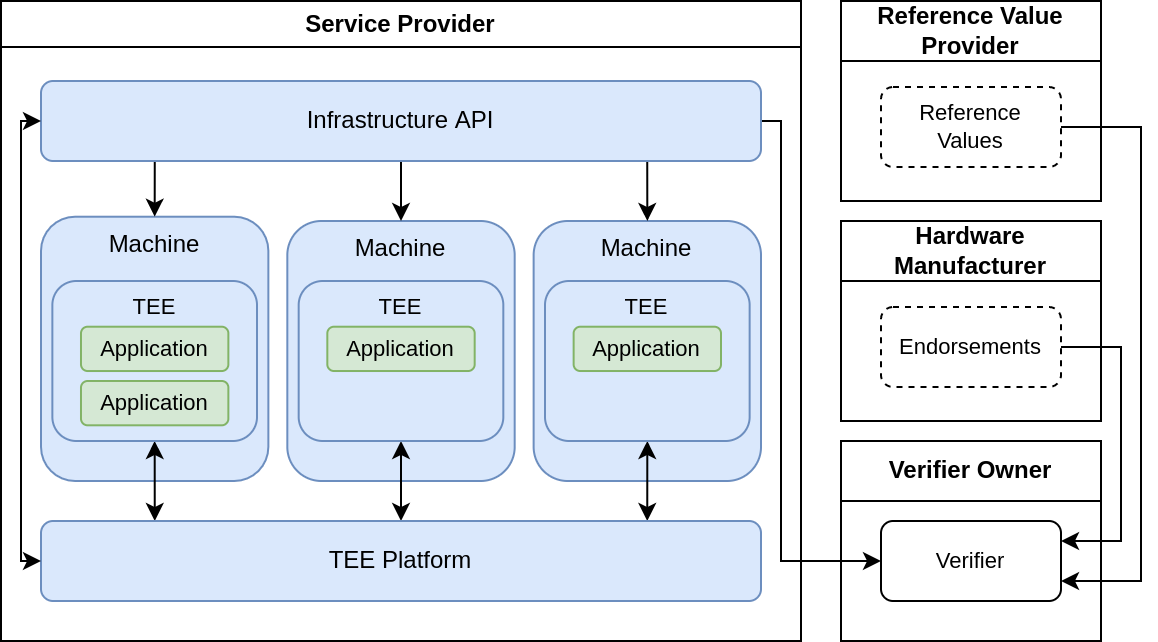
\includegraphics[width=0.9\linewidth]{resources/untrusted-infrastructure-architecture.drawio.png}
  \caption{Overview of the infrastructure in the trusted distributed computing model.}
  \label{fig:untrusted-architecture-overview}
\end{figure}

As outlined in the threat model, protection of data resting in storage resources
and traversing network resources has to be implemented at application level
using authentication, authorization, and encryption.

Instead of directly running applications on provided (physical or virtual)
machines, the data and application owner rely on TEEs to protect data that is
currently in use by applications. In Section \ref{sec:confidential-computing} we
have seen two TEE models. On one hand, a service provider can provide machines
capable of creating process-based TEEs inside those machines, on the other hand,
a service provider can also provide VM-based TEEs, in which case the machine
itself is the TEE.

The TEE platform has to be capable to produce evidence of software components
that have direct access and/or control the access to the memory of a TEE, such
as VM firmware and firmware components of the TEE platform. While the TEE
platform is operated by the service provider, the TEE platform is provided to
the service provided and endorsed by the hardware manufacturer.

A secure channel is essential for data owners to supply applications inside TEEs
with confidential data. Section \ref{sec:ra-secure-communication-channel}
outlined the basic process of establishing a secure communication channel
between the attester and the relying party during the remote attestation
process.

\subsection{Platform Layer}

Like in the traditional distributed computing model, the Platform layer builds
on top of the Infrastructure layer. Therefore, this section assumes the presence
of a TEE platform that can be used to securely deploy applications and provide
the application with confidential data.

Because in this model the service provider is untrusted, there are three
possible solutions to the issues of the services typically located in the
Platform layer:

\begin{itemize}
  \item Moving these services to the Application layer or directly implementing
        the tasks that these services take on into applications.
  \item Management of the service by a trusted party that is not the application
        owner (otherwise it would mean that the service is in the application
        layer).
  \item Splitting the service into a privileged and unprivileged part. The
        unprivileged part can still be operated by the service provider, while
        the privileged part has to be managed by the application owner.
\end{itemize}

The first option can be applied to all services of the Platform layer, as such
this section will focus on the evaluation of each previously defined service
type based on the latter two options.

\begin{description}[style=standard]
  \item[Infrastructure Management Services] do not need to be modified and can
    still be managed by the service provider, assuming applications are
    adequately shielded from Infrastructure layer resources as described in the
    previous section.

  \item[Security Services] can not be managed by an untrusted party, as
    application-level security depends on those services. Management of
    identities, administration of authentication policies, and encryption and
    decryption of data are all privileged tasks. Therefore, splitting security
    services into unprivileged and privileged parts is not feasible and these
    services have to managed by a trusted party.

  \item[Monitoring and Logging Services] can be managed by a service provider,
    assuming that application logs do not include sensitive information or are
    protected (e.g. encrypting or obfuscating logs).

  \item[Application Orchestration Services] are a more complex topic. Because
    the TEE platform is still under control of the service provider, software
    responsible for managing TEEs are still untrusted (e.g. hypervisor, OS
    managing process-based TEEs). Applications and application configurations
    can also be modified by an attacker during the deployment of applications
    into TEEs. Therefore, TEEs, applications, and application configurations
    have to be verified before supplying applications with confidential data.

    There are two ways on how applications can be deployed into TEEs:

    The first option is to create an application package that can be directly
    deployed by the TEE platform. For example the application owner might
    package an application including its (non-confidential) configuration
    directly into an VM image that can be deployed by the service provider. The
    application owner has to provide reference values in the form of
    measurements of the VM, in order for the verifier to verify the integrity of
    the VM including the applications inside. This option moves the installation
    and configuration of applications into the application packaging process,
    and therefore requires a more complex packaging solution. However, it also
    allows the combined verification of TEEs, applications, and application
    configurations.

    The second option is to first create a generic application-agnostic TEE and
    subsequently deploy the application including its (non-confidential)
    configuration into the TEE after verifying its integrity. For example a
    service provider might provide a curated list of generic VM images that can
    be deployed by tenants as VM-based TEEs. A reference value provider has to
    deploy such a VM image, check its content for malicious software, and create
    measurements of the VM beforehand, producing reference values. After a
    VM-based TEE is created, the verifier has to verify the integrity of the
    VM-based TEE using the reference values, after which the application owner
    installs, configures, and executes applications in the verified VM. This
    option decouples the creation of TEEs from the installation, configuration,
    and execution of applications, allowing another reference value provider to
    maintain reference values for TEEs. However, this also decouples the
    verification of TEEs from the verification of applications and their
    configurations, requiring two separate verifications.

    While in both cases the service provider creates TEEs, the service provider
    is not involved in the installation, configuration, and execution of
    applications in the provided TEEs. Both options also require a secure way to
    supply the applications with confidential data, which can again be achieved
    by establishing a secure communication channel during the remote attestation
    process.
\end{description}

\subsection{Application Layer}

The threat model above already discussed how application level authentication,
authorization, and encryption of confidential data is crucial to protect data
resting in storage resources and traversing network resources. As the service
provider is not trusted, Infrastructure and Platform layer protection methods
can not be used, and the application owner has to implement these protections
into the Application layer.

\section{Requirements}
\label{sec:requirements}

This section summarizes the changes made to the traditional distributed
computing model and defines requirements for the trusted distributed computing
model.

The trusted distributed computing model is largely based on concepts of the
confidential computing model and requires a hardware manufacturer to provide:

\begin{enumerate}[label*=R\arabic*]
  \item a TEE platform, capable of creating TEEs and generating evidence, based
        on hardware mechanisms.
  \item endorsements that vouch for the TEE platform's capability to securely
        generate evidence and protect the confidentiality and integrity of TEEs.
\end{enumerate}

There are two requirements for the offerings of a service provider. The service
provider has to provide:

\begin{enumerate}[resume,label*=R\arabic*]
  \item the ability to create TEEs using the TEE platform provided by the hardware
        manufacturer.
  \item the raw evidence produced and signed by the TEE platform that includes:
        \begin{enumerate}[label*=.\arabic*]
          \item measurements of the content of the TEE.
          \item measurements of software components that have direct access or
                the access to the memory TEEs.
        \end{enumerate}
\end{enumerate}

The latter requirement enables the verifier to verify TEEs, preventing the
service provider to tamper with provided TEEs in order to break the
confidentiality and integrity guarantees. This leads to the requirements for the
verifier. The verifier has to verify

\begin{enumerate}[resume,label*=R\arabic*]
  \item the integrity of provided TEEs using measurements provided by the
        service provider and reference values from the reference value provider.
  \item the integrity of the TEE platform by verifying:
        \begin{enumerate}[label*=.\arabic*]
          \item the authenticity of the evidence using the evidence's signature
                and endorsements from the hardware manufacturer.
          \item the integrity of software components that have direct access or
                control the access to the memory of TEEs using measurements of
                those components and reference values from a reference value
                provider.
        \end{enumerate}
\end{enumerate}

While TEEs protect data currently in use by applications, data resting in
storage resources and traversing network resources also have to protected. The
application management process also has to be secured, preventing the service
provider to execute malicious applications inside TEEs and modifying
applications before they are deployed into TEEs. This results in the following
requirements for the application owner. The application owner has to:

\begin{enumerate}[resume,label*=R\arabic*]
  \item implement security (authentication, authorization, and encryption) in
        the Application layer, not relying on security services provided by the
        Platform layer.
  \item protect application logs by removing, encrypting, or obfuscating
        confidential information from the logs.
  \item deploy applications inside TEEs. This includes:
        \begin{enumerate}[label*=.\arabic*]
          \item providing reference values for applications and their
                configuration.
          \item installing, configuring, and executing applications inside TEEs.
          \item securely supplying applications with confidential data only
                after verification of applications and their surrounding TEE
                (e.g. by establishing a secure communication channel during the
                remote attestation process).
        \end{enumerate}
\end{enumerate}

%%%%%%%%%%%%%%%%%%%%%%%%%%%%%%%%%%%%%%%%%%%%%%%%%%%%%%%%%%%%%%%%%%%%%%%%%%%%%%%%
% Evaluation
%%%%%%%%%%%%%%%%%%%%%%%%%%%%%%%%%%%%%%%%%%%%%%%%%%%%%%%%%%%%%%%%%%%%%%%%%%%%%%%%

\section{Evaluation}
\label{sec:evaluation}

This section evaluates the requirements of the trusted distributed computing
model based on the threat model defined in section
\ref{sec:untrusted-threat-model}.

Infrastructure layer threats from storage and network resources are addressed in
the trusted distributed computing model by R7. By implementing authentication,
authorization, and encryption at application level, an attacker that gained
access to storage and network resources or the untrusted service provider
providing these resources, still do not have plain text access to confidential
data.

Threats from compute resources of the Infrastructure layer are addressed by
R1-R6. The issue of traditional mitigations of these threats was the lack of a
trusted component that can verify the integrity of components that implement the
mitigations. R3 and R4 require the service provider to offer the capability to
create TEEs using and get evidence produced and signed by a TEE platform. The
TEE platform is provided and endorsed by the hardware manufacturer (R1 and R2).
Section \ref{sec:confidential-computing} described how TEEs protect memory
confidentiality and integrity using memory encryption and access control.

Physical access to a machine's memory (DMA and PME attacks) are prevented as
data leaving the CPU is encrypted before storing it in memory. As such, an
attacker with direct access to a machine's memory still does not have plain text
access to the data.

Virtualization-based attacks are also mitigated by the TEE platform. VM-based
TEEs split of the memory access control and isolation part of the hypervisor of
into the TEE platform. The hypervisor is still provided with interfaces in order
to manage VMs (e.g. starting, stopping, suspending), but the isolation guarantee
is provided by the TEE platform. And while the hypervisor is also tasked with
managing VM memory (e.g. attaching and releasing), the hypervisor can not read
the memory as it is encrypted.

Measurements produced by the TEE platform can also be used for the measured boot
process mitigating BI attacks against VM-based TEEs. Ongoing work in QEMU, an
open source emulator that can facilitate hardware-assisted virtualization in
order to run VMs, the open virtual machine firmware (OVMF), and the Linux kernel
enable the verification of all components involved in the boot process of an AMD
SEV based VM (see Section \ref{sec:commercial-tee-technologies}). The basic boot
process works as follows: When a VM is started, the AMD-SP measures the VM's
firmware (OVMF), which in turn measures and verifies the integrity of the Linux
kernel. After the VM has booted, the Linux kernel is supplied with an
attestation report that contains a measurement of OVMF, which are relayed to the
verifier in order to verify OVMF's integrity. The attestation report also
contains evidence about the integrity of SEV's firmware components which
together with the measured boot process fulfill requirements R4, allowing a
verifier that supports the verification of SEV's attestation report to fulfill
R5 and R6.

The TEE creation capability of process-based TEE platforms can often be passed
through to VMs (e.g. in the case of Intel SGX), in which case the VM itself and
the hypervisor are not considered trusted. Again, isolation is provided by the
TEE platform (R3), and not the hypervisor. In this model, compromising the VM on
which the process-based TEE is deployed only threatens the availability of the
application, and not the confidentiality of the application's data. TEE
platforms based on the process-based TEE model, still need to provide
measurements of software components of the TEE platform and the TEEs (R4),
allowing a verifier to verify the integrity of the TEE platform (R6) and TEEs
(R5).

R7 requires the implementation of security mechanisms in the Application layer.
These mechanisms can not be based on security services provided by the Platform
layer, as this would allow spoofing and elevation of privilege attacks, or plain
text access to confidential data from the untrusted service provider. While R8
does not require moving monitoring and logging services into the application
layer, it does require the Application layer to protect sensitive information in
application logs. Infrastructure management services can still be part of the
Platform layer, as confidential is already protected from Infrastructure layer
resources by R1-R7.

Application orchestration however, still relies on management of target
environments for applications to be managed by untrusted software components.
That is VM-based TEEs managed by a hypervisor or process-based TEEs managed by
the surrounding host (or guest) OS. R9 requires that the rest of the application
orchestration process, that is installation, configuration, and execution of
applications inside provided target environments, is managed by the application
owner. It also requires the verification of both TEEs and applications before
supplying applications with confidential data. Requiring the verification of
applications enables the detection of modification of applications or their
configurations, and requiring the application owner to manage the execution of
applications inside verified TEEs, prevents the service provider to execute
malicious code.

On the one hand, all R7-R9 remove the service provider as a trusted party, but
on the other hand they significantly increase the responsibilities of
application owners and the size of the Application layer.

%%%%%%%%%%%%%%%%%%%%%%%%%%%%%%%%%%%%%%%%%%%%%%%%%%%%%%%%%%%%%%%%%%%%%%%%%%%%%%%%
% Case Studies
%%%%%%%%%%%%%%%%%%%%%%%%%%%%%%%%%%%%%%%%%%%%%%%%%%%%%%%%%%%%%%%%%%%%%%%%%%%%%%%%

\section{Case Studies}
\label{sec:case-studies}

\subsection{Case Study: Constellation}

Constellation is a project maintained by Edgeless
Systems\footnote{\url{https://docs.edgeless.systems/constellation/}}. By
extending Kubernetes, Constellation provides a platform base that includes
infrastructure management and application orchestration services (see Section
\ref{sec:example-kubernetes}) on top of the Infrastructure layer provided by an
untrusted cloud provider. Its contribution is the protection of the whole
Kubernetes cluster from underlying Infrastructure layer resources by utilizing
VM-based TEEs, and providing transparent network and storage encryption.

\begin{figure}[H]
  \centering
  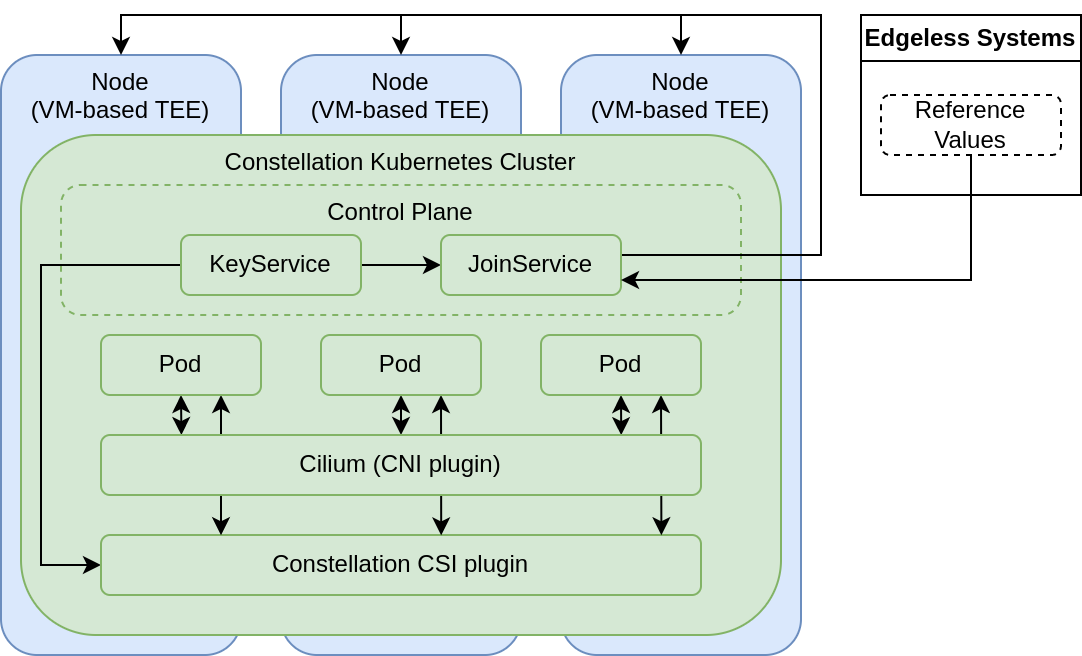
\includegraphics[width=0.8\linewidth]{resources/constellation-kubernetes.drawio.png}
  \caption{Constellation Kubernetes overview.}
\end{figure}

In order to protect data currently in use by control plane components and
application pods, Constellation runs the whole cluster on VM-based TEEs. The
JoinService, a new component of the control plane, is responsible for verifying
new nodes joining the cluster. After a node that is supposed to run control
plane components is verified and joins the cluster, it is supplied by the
JoinService with encryption keys supplied by the KeyService. These keys are then
used to encrypt etcd data that is stored on the node, protecting control plane
data at rest.

In this architecture, the JoinService correlates to the verifier introduced
previously. It uses reference values provided by Edgeless Systems in order to
verify joining nodes. The KeyService manages cryptographic keys used for
encryption and decryption and is therefore a security service.

Protection of control plane and application data in transit is provided by
cilium, the CNI plugin chosen by constellation, which encrypts data exchanged
between pods without the need for applications running inside pods to be
modified. Persistent application data at rest is shielded by the CSI plugin
provided by Constellation, which encrypts and decrypts persistent volumes using
keys provided by the KeyService without needing modification of the applications
inside pods. Both the CNI and the CSI plugin are implementations of
infrastructure and security services

Constellation currently only supports AMD SEV, making AMD take on the role of
hardware manufacturer that provides and endorses the TEE platform (R1 and R2).
However, the currently supported cloud providers (Azure, GCP, AWS) do not fully
support the trusted distributed computing model at the time of writing. For
example AWS currently does not provide the capability of providing SEV based
VMs, not meeting R3. While Azure and GCP provide SEV based VMs, Azure currently
does not provide reviewable VM firmware, not meeting R4.2, and GCP does not
provide evidence produced by the SEV platform, not meeting R4.

Because the cloud providers do not meet R3 and R4, the verifier in the
Constellation architecture (JoinService) can not fulfill R5 and R6. On the one
hand, if the cloud provider does not meet R3, there are no TEEs to be verified,
making complying with R5 impossible. On the other hand, if the cloud provider
does not meet R4, the verifier can not fully verify the integrity of the TEE
platform or TEE, preventing the verifier to satisfy R6.

While Edgeless Systems provides application owners with tools to create and
manage a Constellation Kubernetes cluster, the cluster still has to be
administered by the application owner, putting the whole cluster into the
Application layer. In doing so Constellation meets requirements R7 and R9,
because security services (KeyService, CNI, and CSI plugin) and application
orchestration services (natively included in Kubernetes) are now managed by the
application owner.

\subsection{Case Study: Confidential Containers}

Confidential Containers is another project, trying to implement the untrusted
distributed computing model into the Kubernetes
architecture\footnote{\url{https://github.com/confidential-containers/documentation}}.
The key difference, is that while Constellation applies confidentiality at the
node level, Confidential Containers applies confidentiality at a pod level. By
running containers inside TEEs (both VM-based and process-based) and not the
whole cluster, Confidential Containers goal is to separate the trust model of
the Kubernetes cluster from the applications deployed in the cluster. The
project is still in a very early development stage, as such information provided
in this section is subject to change.

The current Kubernetes architecture puts the container runtime in charge of
managing pods and containers inside the pod (see Section
\ref{sec:example-kubernetes}). Confidential Containers introduces a new
component into the pod: the enclave agent. The enclave agent collects claims
generated by the TEE platform, performs the remote attestation process, receives
confidential configuration and data, pulls container images from the container
image registry, and manages the lifecycle of containers inside the pod. In the
case of VM-based TEEs, a pod is represented by a single VM, which includes the
enclave agent as a process that is started at boot and the containers are
started inside the VM. For process-based TEEs, the enclave agent is a separate
process-based TEE, that creates distinct process-based TEEs for each container
on the node itself. In this case study we will illustrate the Confidential
Container architecture only using VM-based TEEs.

\begin{figure}[H]
  \centering
  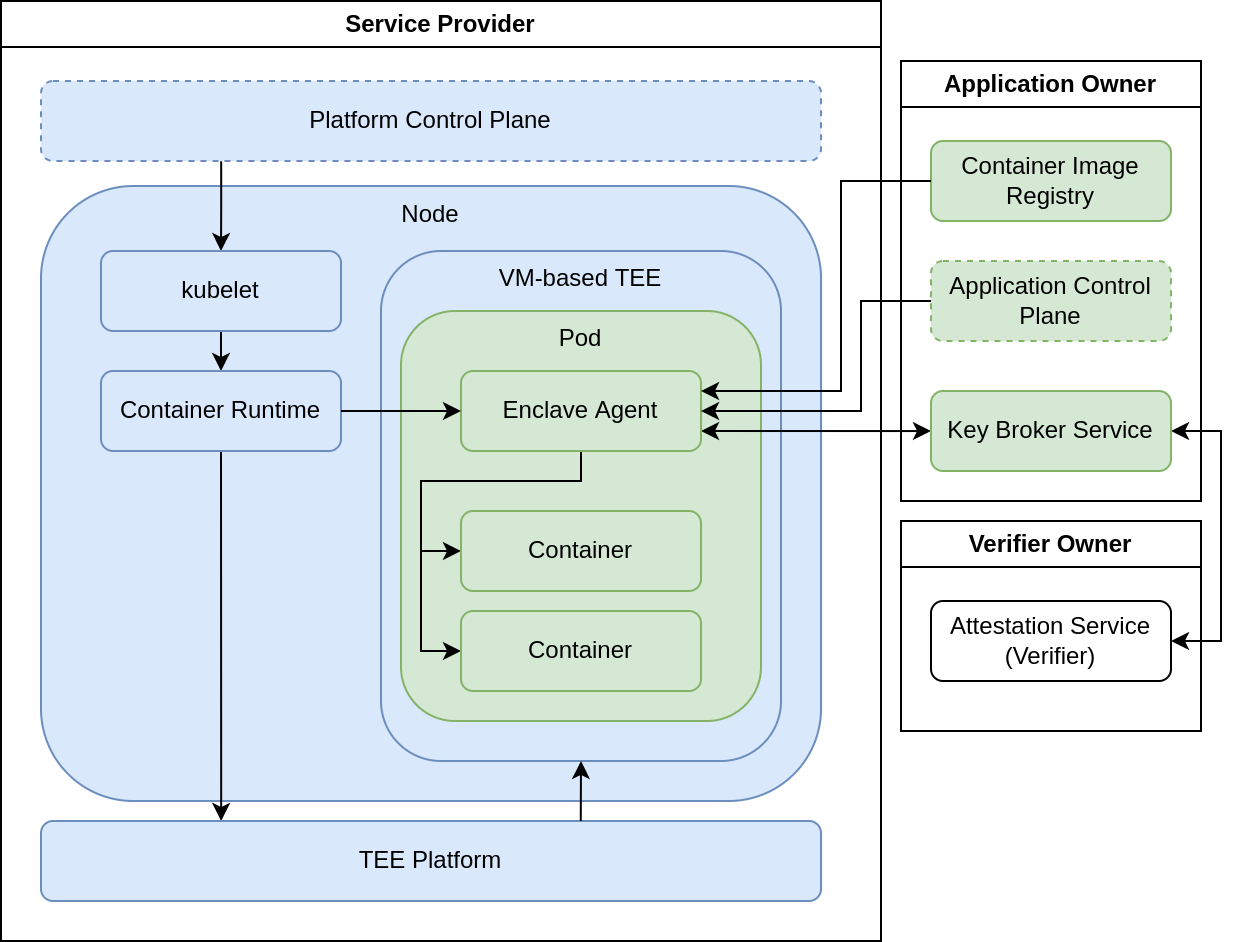
\includegraphics[width=0.8\linewidth]{resources/confidential-containers.drawio.png}
  \caption{Confidential Containers application orchestration overview.}
\end{figure}

While the agent only acts upon request from a single API source, traditionally
the Kubernetes control plane, Confidential Containers is currently working on
splitting the Kubernetes control plane into a trusted and an untrusted part. The
platform control plane (untrusted) would be responsible for unprivileged tasks,
such as infrastructure and TEE management. On the other hand, the application
control plane (trusted) performs privileged tasks, including container
management inside TEEs provided by the platform control plane. The split of the
control plane is enforced by the enclave agent, by blocking privileged actions
originating from the platform control plane, such as creating a malicious
container in a pod, and establishing a secure communication channel to the
application control plane.

The architecture builds upon the assumption that confidential data is provided
to the pod using persistent volumes managed by a CSI plugin, but stored in an
encrypted form. Decryption keys are provided to pods by the key broker service,
which correlates to the relying party of the RATS framework. It receives
evidence from the enclave agent, relays the evidence to the verifier (called
attestation service in the Confidential Containers architecture) for
verification, applies appraisal policies on the returned attestation results,
and releases keys to the enclave agent. During the remote attestation process, a
secure communication channel between the key broker service and the enclave
agent is established, which is used for the secure release of keys to the
enclave agent. Besides data decryption keys the key broker service also sends
communication keys to the enclave agent that are used to establish a secure
communication to other components, such as the application control plane.

Currently, it is still not clear, how the ConfigMap and Secret resources of the
traditional Kubernetes architecture fit into this new architecture, which is why
the following illustration of the application orchestration process does not
include ConfigMaps and Secrets.

\begin{enumerate}
  \item Upon request of a tenant, the platform control plane requests the
        kubelet of a node to create a pod and provides the kubelet with the
        specification of the pod. This specification mainly includes container
        images, storage configuration, and network configuration.
  \item Kubelet calls the container runtime to create the pod and configure its
        storage and network.
  \item The container runtime in turn calls the TEE platform to create a
        VM-based TEE using a predefined VM image that includes the enclave
        agent.
  \item During the boot of the VM the TEE platform produces signed evidence that
        is then passed to the enclave agent after the VM has fully booted. The
        container runtime also passes the pod specifications to the enclave
        agent.
  \item The enclave agent requests the release of keys from the key broker
        service and includes the evidence in the request.
  \item The key broker service relays the evidence to the attestation service
        and receives an attestation result, upon which the key broker service
        applies its own appraisal policy.
  \item If the attestation was successful, the key broker service releases keys
        and a pod specification policy to the enclave agent. The policy can for
        example include storage and network configuration, a container image
        whitelist, a certificate which can be used to validate the authenticity
        of container images.
  \item The enclave agent then compares the pod specification it received from
        the container runtime to the policy. If the specification passes the
        policy, the enclave agent pulls the specified container images and
        validates the signature using the certificate included in the policy.
  \item Only after passing the policy the enclave agent creates the containers
        inside the VM and provides them with decryption keys.
\end{enumerate}

Note that the enclave agent is only trusted, because it is included in the VM
image which is verified by the verifier. Modification of the enclave agent (or
any other software in the VM image) would fail the verification and lead to the
key broker service not releasing keys to the enclave agent.
